\textbf{Behavior-Regularized Offline RL. }We formalize the task as a Markov Decision Process (MDP) $\langle\mathcal{S}, \mathcal{A}, T, R, \gamma\rangle$, where $\mathcal{S}$ is the state space, $\mathcal{A}$ is the action space, $T(s'|s, a)$ denotes the transition function, $R(s, a)$ is a bounded reward function, and $\gamma$ is the discount factor. In offline RL, an agent is expected to learn a policy $\pi: \mathcal{S}\rightarrow \Delta(\mathcal{A})$ to maximize the expected discounted return $\mathbb{E}_{\pi}[\sum_{t=0}^\infty\gamma^tR(s_t, a_t)]$ with an offline dataset $\mathcal{D}=\{(s_t,a_t,s_{t+1},r_t)\}$, where $s_t, s_{t+1}\in\mathcal{S}$, $a_t\in\mathcal{A}$, and $r_t=R(s_t,a_t)\in\mathbb{R}$. 
We consider the behavior-regularized RL objective, which augments the original RL objective by regularizing the policy towards some behavior policy $\nu$:
\begin{equation}\label{eq:brl_obj}
    \begin{aligned}
    \resizebox{0.95\linewidth}{!}{$
        \max_{\pi}\ \mathbb{E}_{\pi}\left[\sum_{t=0}^\infty\gamma^t(r_t-\eta\KL{\pi(\cdot|s_t)}{\nu(\cdot|s_t)})\right],
        $}
    \end{aligned}
\end{equation}
where $D_{\rm KL}$ is the Kullback-Leibler (KL) divergence and $\eta>0$ controls the regularization strength. In offline RL, \eqref{eq:brl_obj} is widely employed by setting $\nu$ as the policy $\pi_{\mathcal{D}}$ that collects the dataset to prevent the exploitation of the out-of-dataset actions. Besides, when setting $\nu$ as the uniform distribution, \eqref{eq:brl_obj} equates to the maximum-entropy RL in online scenarios up to some constant. 

To solve \eqref{eq:brl_obj}, a well-established method is soft policy iteration~\citep{sac,brac}. Specifically, we define the soft value functions as
\begin{equation}\label{eq:expected_q}
    \begin{aligned}
        V^\pi(s)=\mathbb{E}_\pi\left[\sum_{t=0}^\infty\gamma^t\left(r_t-\eta\log\frac{\pi(a_t|s_t)}{\nu(a_t|s_t)}\right)\right], 
    \end{aligned}
\end{equation}
where the expectation is taken w.r.t. random trajectories generated by $\pi$ under the initial condition $s_0=s$ and $a_0=a$. The soft $Q$-value function in this framework can be solved by the repeated application of the soft Bellman operator $\mathcal{B}^\pi$:
\begin{equation}\label{eq:expected_bellman}
    \begin{aligned}
        \mathcal{B}^\pi Q^\pi(s, a)=R(s, a)+\gamma \mathbb{E}\left[Q^\pi(s', a')-\eta \log \frac{\pi(a'|s')}{\nu(a'|s')}\right],
    \end{aligned}
\end{equation}
where $s'\sim T(\cdot|s, a)$ and $a'\sim\pi(\cdot|s')$.
For policy improvement, we can update the policy using the objective:
\begin{equation}\label{eq:expected_pi}
    \begin{aligned}
        \max_{\pi}\ \mathbb{E}_{a\sim \pi(\cdot|s)}\left[Q^\pi(s, a)\right] - \eta\KL{\pi(\cdot|s)}{\nu(\cdot|s)}. 
    \end{aligned}
\end{equation}
Note that regularization is added for both $Q$-value functions and the policy. By iterating between policy evaluation and improvement, the performance of the policy defined by \eqref{eq:brl_obj} is guaranteed to improve~\citep{sac}. 


\textbf{Diffusion Models. }Diffusion models~\citep{ddpm,diffusion_sde} consist of a forward Markov process which progressively perturbs the data $x^0\sim q_0$ to data that approximately follows the standard Gaussian distribution $x^N\sim q_N$, and a reverse Markov process that gradually recovers the original $x^0$ from the noisy sample $x^N$. The transition of the forward process $q_{n+1|n}$ usually follows Gaussian distributions:
\begin{equation}
    \begin{aligned}
        q_{n|n-1}(x^{n}|x^{n-1})=\mathcal{N}(x^{n}; \sqrt{1-\beta_{n}}x^{n-1}, \beta_{n}I),
    \end{aligned}
\end{equation}
where $\{\beta_{n}\}_{n=1}^N$ is specified according to the \textit{noise schedule} and $I$ denotes the Identity matrix. Due to the closure property of Gaussian distributions, the marginal distribution of $x^n$ given $x^0$ can be specified as:
\begin{equation}
    \begin{aligned}
        q_{n|0}(x^n|x^0)=\mathcal{N}(x^n; \sqrt{\alphabar_n}x^0, (1-\alphabar_n)I),
    \end{aligned}
\end{equation}
where $\alpha_n=1-\beta_n, \alphabar_n=\prod_{n'=1}^n \alpha_{n'}$. The transition of the reverse process can be derived from Bayes' rule, 
\begin{equation}
    \begin{aligned}
        q_{n-1|n}(x^{n-1}|x^{n})=\frac{q_{n|n-1}(x^{n}|x^{n-1})q_{n-1}(x^{n-1})}{q_{n}(x^{n})}.
    \end{aligned}
\end{equation}
However, it is usually intractable, and therefore we use a parameterized neural network $p^\theta_{n-1|n}$ to approximate the reverse transition, which is also a Gaussian distribution with parameterized mean:
\begin{equation}\label{eq:reverse_diff}
    \begin{aligned}
        p^\theta_N(x^N)&=\mathcal{N}(0, I),\\
        p^\theta_{n-1|n}(x^{n-1}|x^{n})&=\mathcal{N}(x^{n-1}; \mu^\theta_{n}(x^{n}), \sigma^2_{n}I),\\
    \end{aligned}
\end{equation}
where $\sigma_n=\sqrt{\frac{1-\bar{\alpha}_{n-1}}{1-\bar{\alpha}_n}\beta_n}\approx \sqrt{\beta_n}$. The learning objective is matching $p^\theta_{n-1|n}(x^{n-1}|x^{n})$ with the posterior $q_{n-1|n,0}(x^{n-1}|x^{n},x^0)$:
\begin{equation}
\label{eq:elbo}
\scalemath{0.95}{
\begin{aligned}
    &\mathcal{L}_{\rm diff}(\theta) = \\
    &\mathbb{E}_{n,x^0,x^n}\left[\KL{q_{n-1|n,0}(x^{n-1}|x^{n},x^0)}{p^\theta_{n-1|n}(x^{n-1}|x^{n})}\right],
\end{aligned}
}
\end{equation}
where $x^0\sim q_0, x^n\sim q_{n|0}(\cdot|x^0)$. Upon the completion of training, it can be shown that the objective \eqref{eq:elbo} yields 
\begin{equation}
    \begin{aligned}
        p^\theta_{n-1|n}(x^{n-1}|x^n)\approx q_{n-1|n}(x^{n-1}|x^n).
    \end{aligned}
\end{equation}
Simplified training objectives can be derived by reparameterizing $\mu^\theta$ with noise prediction or score networks \citep{ddpm,diffusion_sde}. 
After training, the generation process begins by sampling $\hat{x}^N \sim \mathcal{N}(0, I)$, followed by iteratively applying $p^\theta_{n-1|n}$ to generate the final samples $\hat{x}_0$, which approximately follow the target distribution $q_0$.

\begin{figure}
    \centering
    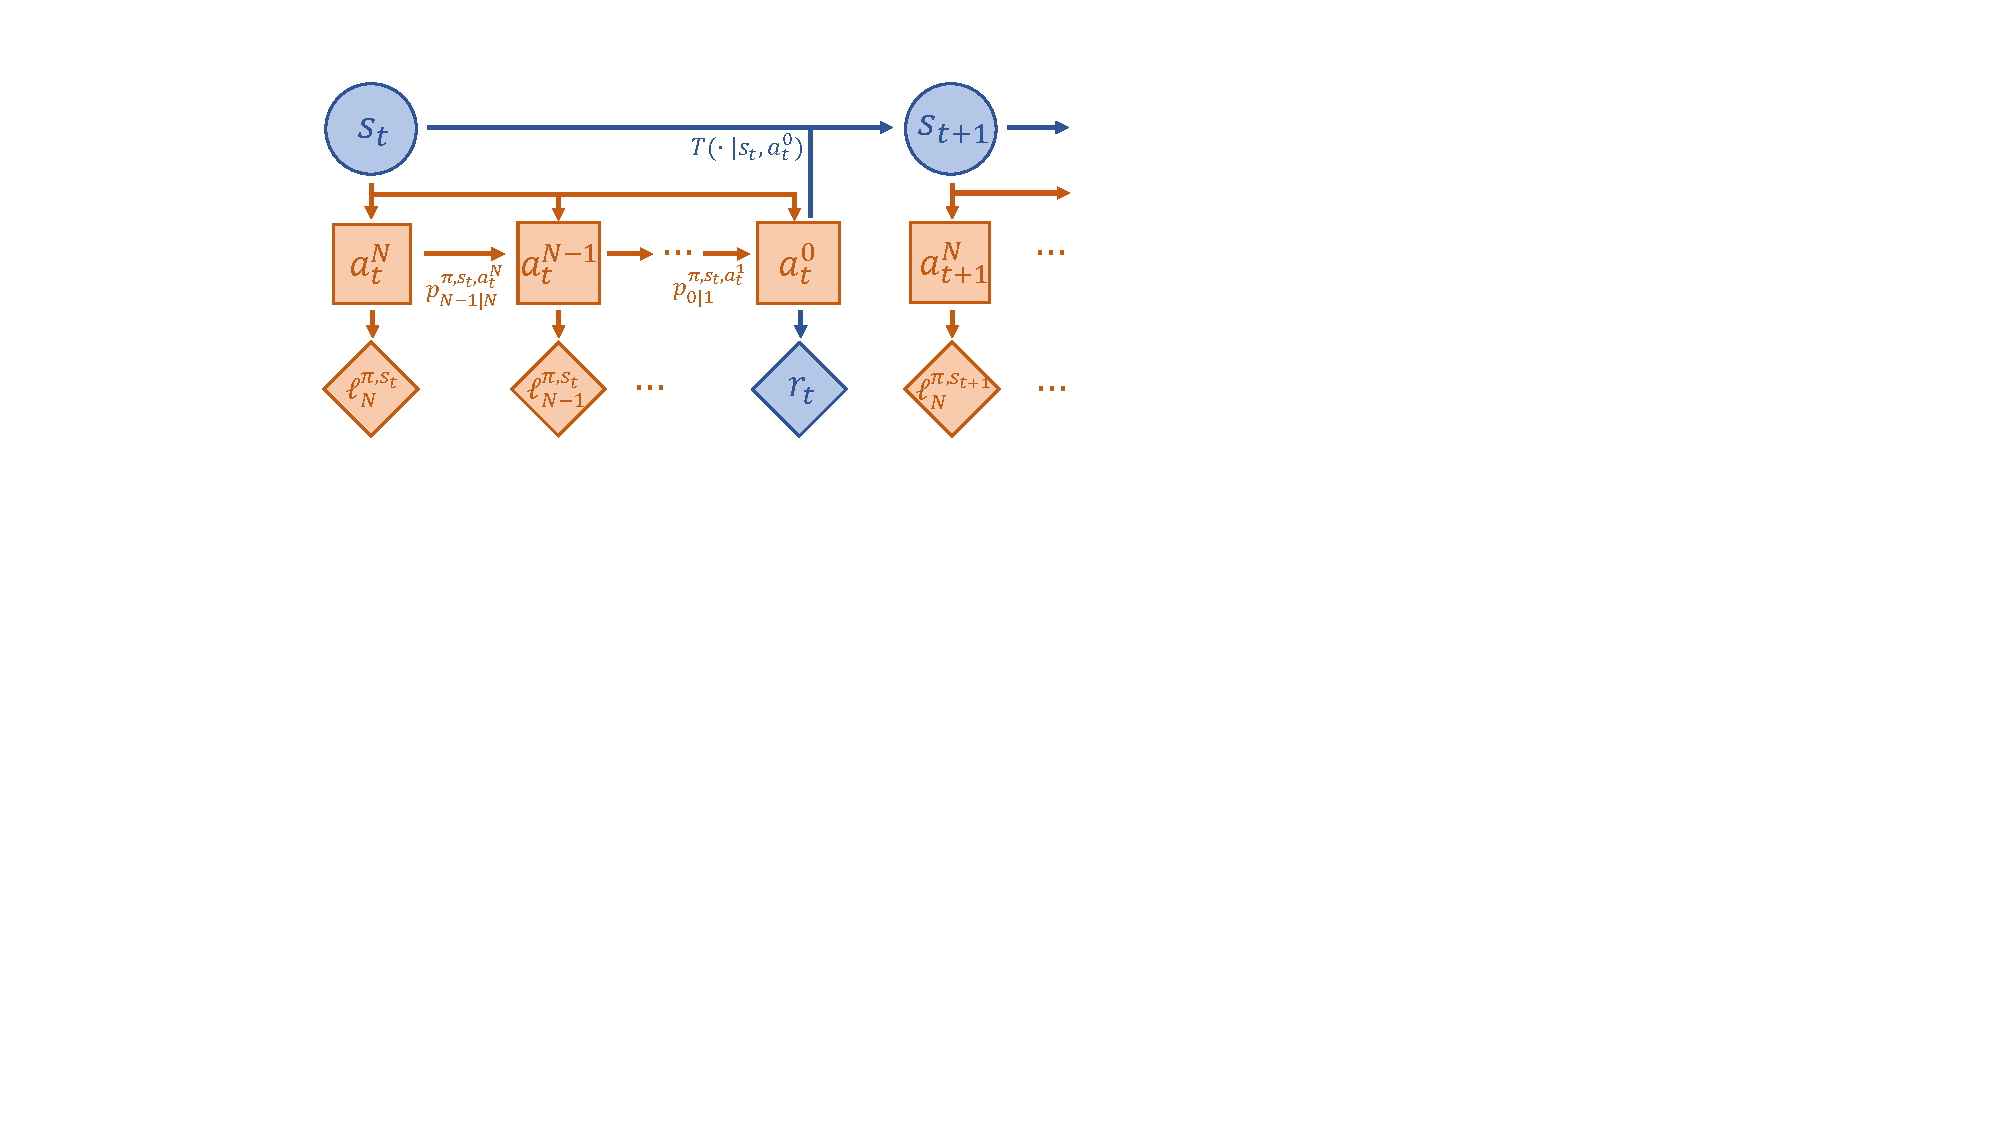
\includegraphics[width=0.9\linewidth]{images/intro_mdp.pdf}
    \caption{Semantic illustration of the interplay between diffusion policies and the environment. We use orange to denote the transition $p_{n-1|n}^{\pi,s_t,a^n}$ and the penalty $\ell_{n}^{\pi,s_t}$ (see Section~\ref{sec:pathwise_kl}) associated with the diffusion generation process, whereas blue signifies the transition $T(\cdot|s_t,a_t^0)$ and the reward $r_t$ from the original environment MDP.}
    \label{fig:intro_mdp}
    \vspace{-3mm}
\end{figure}

\textbf{Diffusion Policy. }Diffusion policies are conditional diffusion models that generate action $a$ on a given state $s$. In this paper, we will use $p^\pi$ and $p^{\pi, s}$ to denote the diffusion policy and its state-conditioned version, respectively. Similarly, we will use $p^{\pi,s,a^n}_{n-1|n}$ as a shorthand for the single-step reverse transition conditioned on $a^n$, i.e., $p^{\pi,s,a^n}_{n-1|n}=p^{\pi,s}_{n-1|n}(\cdot|a_n)$. At timestep $t$ of the environment MDP, the agent observes the state $s_t$, drives the reverse diffusion process $a^{0:N}\sim p^{\pi,s_t}_{0:N}$ as defined in \eqref{eq:reverse_diff}, and takes $a^0$ as its action $a_t$. For action $a_t^n$, we will use $t$ in the subscript to denote the timestep in the environment MDP, while using $n$ in the superscript to denote the diffusion steps. A semantic illustration of the environment MDP and the reverse diffusion is provided in Figure~\ref{fig:intro_mdp}.
